Med henblik på at gøre brugernes data tilgængelig på grafisk vis, implementeres der \textit{charts} i programmet. Den typiske brugere af programmet er børn og for at give dem et overblik over deres indkomst, skal indkomsten vises med et diagram. Ud over at børnene får et overblik, lærer de også om hvordan man aflæser grafer.
I WPF findes et bibliotek, "WPF-Toolkit", som gør det relativt simpelt at binde data op på et diagram. I det følgende afsnit vises et mindre eksempel på hvordan dette kunne gøres:
I \textit{ViewModel} laves eksempelvis en \textit{Dictionary} som indeholder den data der skal vises;

\begin{lstlisting}
public Dictionary<string, int> ChartList
{get; private set; }
\end{lstlisting}

Og herefter laves en \textit{constructor}

\begin{lstlisting}
public ViewModel()
{
	ChartList = new Dictionary<string, int>();
}
\end{lstlisting}

Det tilhørende XAML ser herefter ud som følgende;

\begin{lstlisting}
chartingToolkit:PieSeries DependentValuePath="Value" IndependentValuePath="Key" ItemsSource="{Binding Path=ChartList}
\end{lstlisting}

Et cirkel-diagram, kunne herefter eksempelvis komme til at se ud som på figur \ref{cirkeldia};

\begin{figure}[H]
\centering
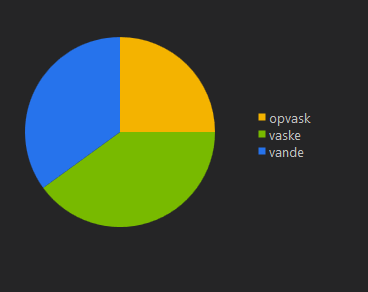
\includegraphics[width=0.6\textwidth]{Billeder/cirkeldia.png}
\caption{Billedet viser hvordan et cirkel-diagram kunne se ud i en C\# application. Fra programmet.}
\label{cirkeldia}
\end{figure}

I programmet vises to forskellige diagrammer, henholdsvis et \textit{LineSeries}-diagram og et \textit{PieSeries}-diagram. Linje-diagrammet viser hvor mange penge brugeren har tjent hver dag over en periode. Cirkel-diagrammet viser brugerens indtjening fordelt på de forskellige pligter vedkommende har udført. Denne data ligger i databasen og hentes ind i to forskellige \textit{Dictionary’s} hvorefter disse kan vises som de to diagrammer. 

